\selectlanguage{ngerman}%
\frenchspacing%
\begin{ledgroupsized}[r]{120mm}%
\footnotesize%
\pstart%
\noindent%
\textbf{Überlieferung:}%
\pend%
\end{ledgroupsized}%
\begin{ledgroupsized}[r]{114mm}%
\footnotesize%
\pstart%
\parindent -6mm%
\makebox[6mm][l]{\textit{L}}%
Aufzeichnung:
LH XXXVII 4 Bl.\;160--161.
Ein Bogen, 4\textsuperscript{o}; %
Ränder beschnitten;
Papiererhaltungsmaßnahmen.
Vier ganzseitig beschriebene Seiten;
geringfügiger Textverlust im Falz von
Bl.\;\href{\Scan{LH_37_04_161v}}{161\,v\textsuperscript{o}}.
Die Aufzeichnung N.\;\ref{57041} setzt den Text von N.\;\ref{57040} unmittelbar fort.
\pend%
\end{ledgroupsized}%
\selectlanguage{latin}%
\frenchspacing%
\vspace*{5mm}%
\normalsize%
\pstart%
\noindent%
\lbrack%
\href{\Scan{LH_37_04_160r}}%
{160\,r\textsuperscript{o}}%
\rbrack%
\phantom{Octobris 1677}%
\hfill%
\phantom{\lbrack160\,r\textsuperscript{o}\rbrack}%
Octobr.\;1677%
\pend%
\vspace{-0.35em}%
\pstart%
\noindent%
\centering{%
\edtext{M.\;P.%
\indexS{motus perpetuus}%
}{%
\lemma{M.\;P.\,}%
\Cfootnote{\textit{motus perpetuus}.%
}}
per Thermom.%
\indexS{thermometrum}
Barometr.%
\indexS{barometrum}
Hygrometr.%
\indexS{hygrometrum}%
\\
\edlabel{LH_37_04_160-161_160r_krd_1a}%
Scheda 1%
\indexS{scheda}%
}%
\edtext{}{%
\xxref{LH_37_04_160-161_160r_krd_1a}{LH_37_04_160-161_160r_krd_1b}%
\lemma{Scheda 1}%
\Bfootnote{%
\lbrack/\rbrack\
\textit{(1)}\;Absolvi %
\textit{(2)}\;Assecutus sum tandem, %
\textit{(a)}\;quem diu %
\textit{(b)}\;quod diu quaesiveram%
~\textit{L}%
}}%
\pend%
\vspace{0.35em}%
\pstart%
\noindent%
Assecutus sum tandem,
quod diu quaesiveram%
\lbrack,\rbrack%
\edlabel{LH_37_04_160-161_160r_krd_1b}
motum perpetuum utilem vitae%
\indexS{motus perpetuus utilis vitae}%
\indexS{vita} %
in exiguo aeque ac magno valiturum:
non illum quidem
quem ignari quaerunt,%
\indexS{ignarus}
quo fieret
ut eadem vis se ipsa major esset%
\indexS{vis major se ipsa}
nulla nova vi accedente;%
\indexS{vis nova}%
\indexS{vis accedens}
sed eum
quem prudentes optare satis habent,%
\indexS{prudentes}
quo
\edtext{%
molendina%
\indexS{molendinum actum sine aqua, vento aut animalibus}
sine aqua%
\indexS{aqua}
et vento%
\indexS{ventus}
et animalibus%
\indexS{animal}
agantur,%
}{%
\lemma{molendina}%
\Bfootnote{%
\textit{(1)}~instituantur, %
\textit{(2)}~etiam \textlangle ut\textrangle\ %
\textit{(3)}~sine aqua %
\lbrack...\rbrack\ et animalibus %
\bars{alligatis \textit{gestr.}} agantur%
~\textit{L}%
}}
aut horologia portatilia%
\indexS{horologium portatile restitutum sponte sua}
sponte sua restituantur.
De Motu perenni%
\indexS{motus perennis portatilis}
\edtext{%
portatili mox%
}{%
\lemma{portatili}%
\Bfootnote{%
\textit{(1)}~postea %
\textit{(2)}~mox%
~\textit{L}%
}}
dicam,
hunc enim novissime inveni.
Majorem illum vitae utilem%
\indexS{motus perpetuus utilis vitae}
dudum in promtu
\edtext{%
habui.
Et variis quidem modis:
\edlabel{LH_37_04_160-161_160r_molvent-1}%
facilior ille est ac popularior %
qui vento nititur,%
\indexS{motus perpetuus nitens vento}
sed non vento perpetuo%
\indexS{ventus perpetuus}
indiget.%
}{%
\lemma{habui.}%
\Bfootnote{%
\textit{(1)}~Qui vento quidem opus hab %
\textit{(2)}~Et variis %
\lbrack...\rbrack\ vento nititur, %
\textit{(a)}~scilicet ventus fortis %
\textit{(b)}~sed non vento perpetuo indiget.%
~\textit{L}%
}}
\edtext{%
\edtext{%
Nimirum vento flante%
\indexS{ventus flans}
non tantum circumagatur machina,%
\indexS{machina circumacta vento}
sed et subito pondera multa %
aut magna eleventur%
\indexS{pondus elevatum vento}
vel elastra comprimantur;%
\indexS{elastrum compressum vento}
quae pondera aut Elastra
cessante vento,%
\indexS{ventus cessans}%
}{%
\lemma{Nimirum}%
\Bfootnote{%
\textit{(1)}~cum vento elevetur pondus maximum aut %
\textit{(2)}~vento %
\bars{flante non %
\lbrack...\rbrack\ et subito \textit{erg.}} pondera multa, %
\textit{(a)}~quae cessante vento %
\textit{(b)}~aut magna eleventur vel elastra %
\textit{(aa)}~tendantur %
\textit{(bb)}~comprimantur; quae pondera %
\textit{(aaa)}~atq %
\textit{(bbb)}~aut Elastra cessante vento%
~\textit{L}%
}}
paulatim ad naturalem%
\indexS{status naturalis}
\edtext{%
statum redire tentent,%
}{%
\lemma{statum}%
\Bfootnote{%
\textit{(1)}~restituant sese %
\textit{(2)}~rever %
\textit{(3)}~redire tentent%
~\textit{L}%
}}
atque interim machinam animent,%
\indexS{machina animata}
tantisper dum ventus
\edtext{%
rediens%
\indexS{ventus rediens}
nova elevatione%
\indexS{elevatio ponderis vento}
aut compressione%
\indexS{compressio elastri vento}
restitat%
}{%
\lemma{rediens}%
\Bfootnote{%
\textit{(1)}~nondum quidem restituta, %
\textit{(2)}~restitant %
\textit{(3)}~nova elevatione aut compressione %
\textit{(a)}~restitant %
\textit{(b)}~restitat%
~\textit{L}%
}}
ipsa in violentum%
\indexS{status violentus}
agendique capacem.%
\indexS{status capax agendi}%
}{%
\lemma{Nimirum \lbrack...\rbrack\ capacem}%
\Cfootnote{%
Ein \textit{horologium ventaneum perpetuum}, durch welches ein \textit{motus regularis continuus a causa irregularis discontinuata} erzeugt werden soll, hatte Leibniz in Paris entworfen; vgl. \textit{LSB} VIII,\;2 N.\;94.\cite{01472}%
}}
Ita Machina semper satis virium habebit%
\indexS{vis machinae}
ad utiles vitae%
\indexS{effectus utilis vitae}%
\indexS{vita}
\edlabel{LH_37_04_160-161_160r_grz_2a}%
effectus.%
\edtext{}{%
\xxref{LH_37_04_160-161_160r_grz_2a}{LH_37_04_160-161_160r_grz_2b}%
\lemma{effectus.}%
\Bfootnote{%
\lbrack/\rbrack\
\textit{(1)}~Objicit %
\textit{(2)}~Obi %
\textit{(3)}~Objici%
~\textit{L}%
}}
\pend%
\newpage%
\pstart%
Objici%
\edlabel{LH_37_04_160-161_160r_grz_2b}
potest
\edtext{%
ventum aliquando%
}{%
\lemma{ventum}%
\Bfootnote{%
\textit{(1)}~non %
\textit{(2)}~aliquando%
~\textit{L}%
}}
rarum esse.%
\indexS{ventus rarus}
Ponamus ergo singulis mensibus%
\indexS{mensis}
semel tantum spirare ventum
restituendae machinae sufficientem,%
\indexS{machina restituenda}
manifestum
\edtext{%
est %
satis magna esse posse vela%
\indexS{velum latum}
ad magnam venti vim%
\indexS{vis venti}
excipiendam.
Et ventum etiam%
}{%
\lemma{est}%
\Bfootnote{%
\textit{(1)}~tum %
\textit{(2)}~satis magna %
\lbrack...\rbrack\ magnam venti %
\textit{(a)}~exci %
\textit{(b)}~vim excipiendam %
\textit{(aa)}~sed et %
\textit{(bb)}~tum etiam %
\textit{(cc)}~. Et ventum etiam%
~\textit{L}%
}}
mediocrem%
\indexS{ventus mediocris}
continuatione vim maximam
\edtext{%
exercere.
Et ut verbo dicam,%
}{%
\lemma{exercere.}%
\Bfootnote{%
\textit{(1)}~Haud d %
\textit{(2)}~Et ut verbo dicam,%
~\textit{L}%
}}
negari non potest
quovis mense%
\indexS{mensis}
tantam venti vim esse,%
\indexS{vis venti}
ut se dispensetur,
et velut in aerarium%
\indexS{aerarium}
dum eo sit opus recondatur,
fortissimum molendinum%
\indexS{molendinum ventaneum}
continue agere possit.
\edtext{%
Excipietur velis latissimis;%
\indexS{velum latum}
in thesaurum%
\indexS{thesaurus}
vero referetur,
et dispensabitur ponderibus%
\indexS{pondus elevatum vento}
vel Elastris.%
\indexS{elastrum compressum vento}
At%
}{%
\lemma{Excipietur}%
\Bfootnote{%
\bars{autem \textit{gestr.}} velis latissimis; %
\textit{(1)}~dispensabitur et %
\textit{(2)}~at %
\textit{(3)}~in thesaurum %
\bars{vero \textit{erg.}} referetur, et %
\lbrack...\rbrack\ Elastris. At%
~\textit{L}%
}}
inquies vela lata%
\indexS{velum latum}
incommoda erunt,
cum ventus nimis fortis erit.%
\indexS{ventus fortis}
Huic rei remedium%
\indexS{remedium}
in promtu est,
ut vela%
\indexS{velum latum}
ubi ad certum celeritatis pervenerunt gradum%
\indexS{gradus celeritatis}%
\indexS{celeritas velorum molendini}%
\lbrack,\rbrack\
constringantur
sive latitudine imminuantur.
\pend%
\begin{edfigure}[1.75em][1.0em]%
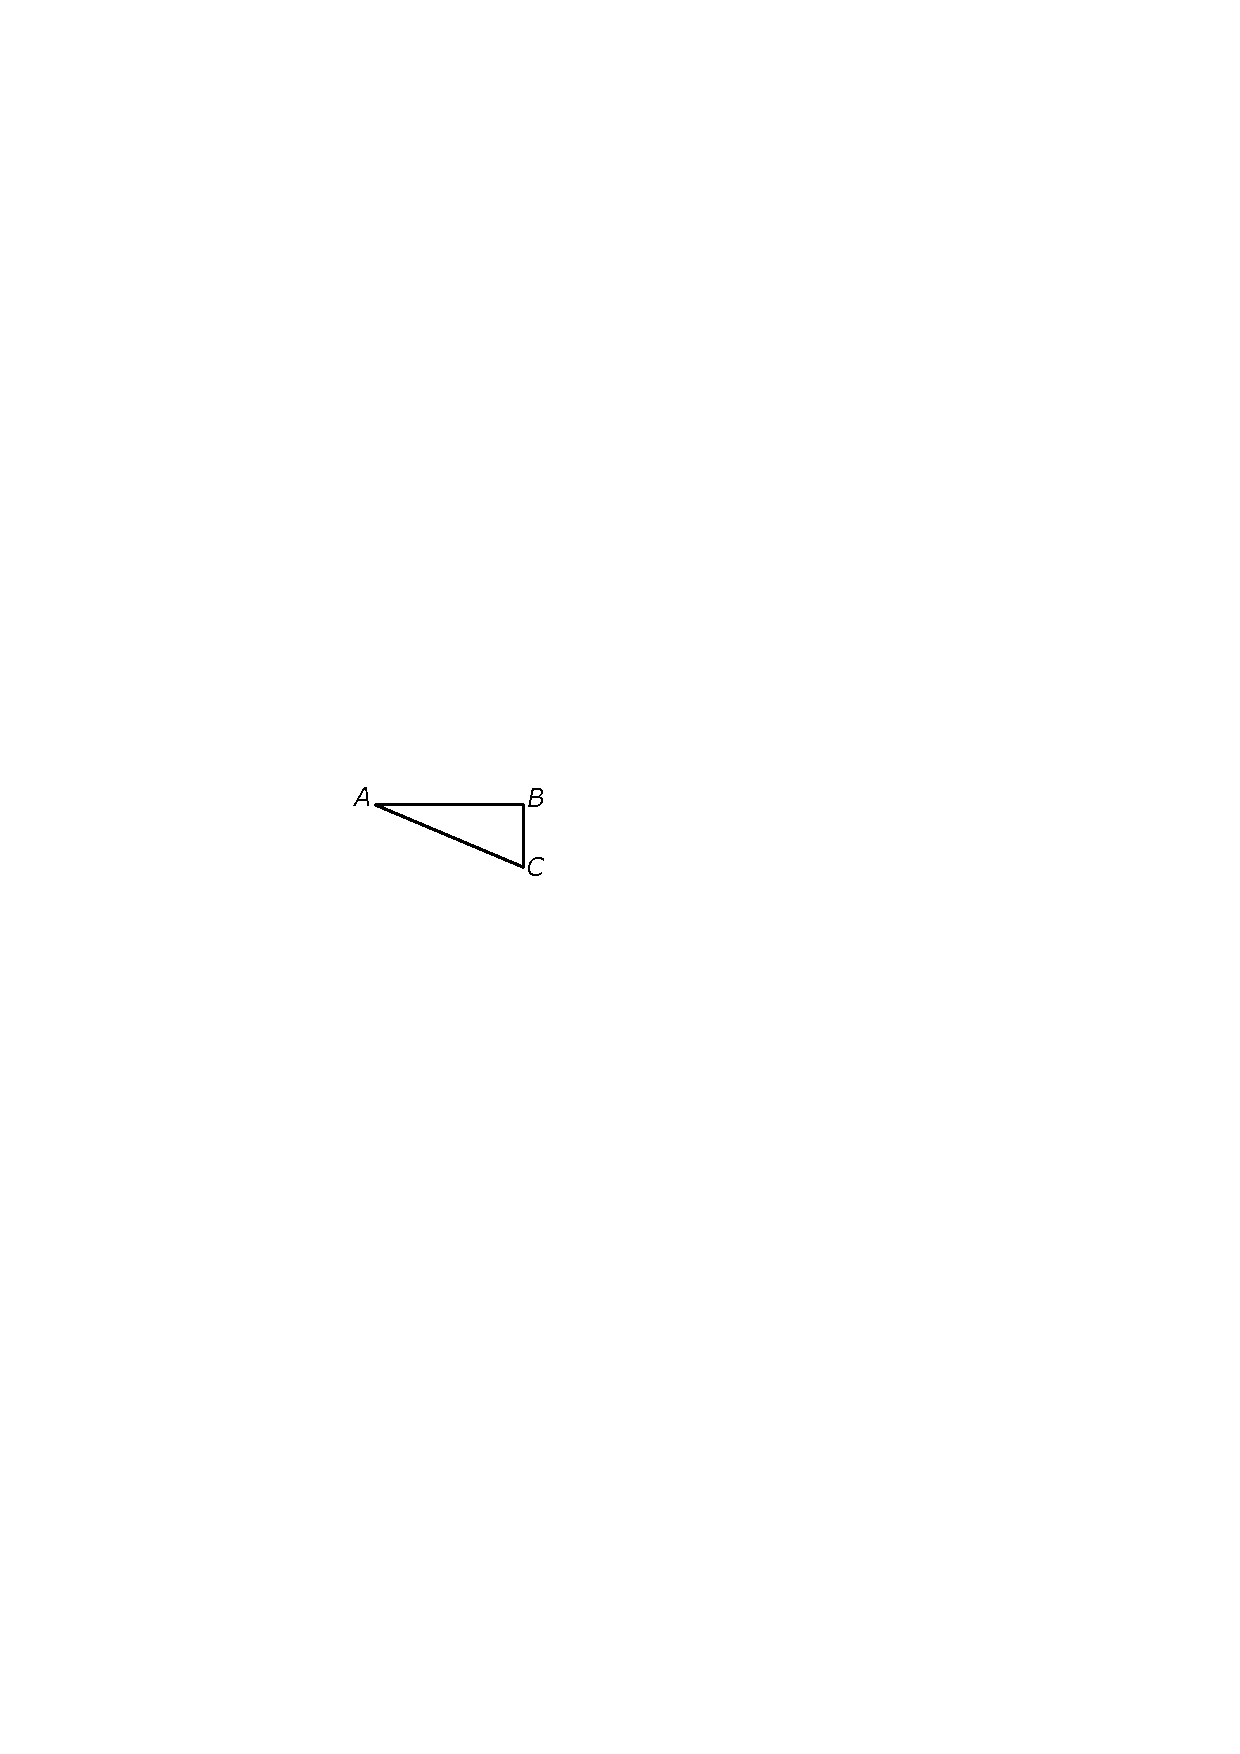
\includegraphics[width=0.20\textwidth]{gesamttex/edit_VIII-4/images/LH_37_04_160-161_d1_160r.pdf}
\edcaption[0.30em]%
{%
\lbrack\textit{Fig.\:1}\rbrack%
\edtext{}{%
\lemma{\lbrack\textit{Fig.\:1}\rbrack}%
\Cfootnote[nonum]{%
In \textit{L} ist das Diagramm im Text eingebunden.%
}}%
}%
\end{edfigure}%
\pstart%
Sed unde tanta copia ponderum%
\indexS{pondus elevatum vento}
atque Elastrorum habebitur,%
\indexS{elastrum compressum vento}
qua vis illa maxima%
\indexS{vis asservata}
satis asservari possit%
\lbrack?\rbrack\
perinde est enim
ac si aquam%
\indexS{aqua agens molendinum}
quae molendinum%
\indexS{molendinum actum aqua}
integro mense agit%
\indexS{mensis}
asservare
\edtext{%
vellemus;
ubi notandum
quod aqua%
\indexS{aqua agens molendinum}
quae molendinum agit%
}{%
\lemma{vellemus;}%
\Bfootnote{%
\textit{(1)}~respondeo aqua quae %
\textit{(a)}~mense %
\textit{(b)}~molendinum mense agit %
\textit{(2)}~praesertim %
\textit{(3)}~ubi notandum %
\lbrack...\rbrack\ molendinum agit%
~\textit{L}%
}}
in magna mole parum habet virium,%
\indexS{moles aquae}%
\indexS{vires in mole}
ob exiguam fluxus%
\indexS{fluxus aquae}
\edtext{%
inclinationem,%
\indexS{inclinatio fluxus aquae}
itaque si defluxus esset perpendicularis,%
\indexS{defluxus perpendicularis}
crederem vix millesima parte%
}{%
\lemma{inclinationem,}%
\Bfootnote{%
\textit{(1)}~itaque videntur integrae vires unius mensis %
\textit{(2)}~itaque si %
\textit{(a)}~flux %
\textit{(b)}~defluxus esset perpendicularis, crederem vix %
\textit{(aa)}~centesima %
\textit{(bb)}~millesima parte%
~\textit{L}%
}}
opus fore.
Ponamus
declivitatem esse \textit{AC},%
\indexS{declivitas fluxus aquae}
altitudinem \textit{BC},
erit ut \textit{AC} ad \textit{BC},
ita ratio virium.%
\indexS{ratio virium}
Quare si \textit{BC} sit pes,%
\indexS{pes}
et \textit{AC} decies mille pedes,
seu si decies
\edtext{%
mille pedum cursu sit opus%
\indexS{cursus}
ad unius pedis depressionem,%
\indexS{depressio}%
}{%
\lemma{mille}%
\Bfootnote{%
\textit{(1)}~pedes sit opus ad unum pedem %
\textit{(2)}~cur %
\textit{(3)}~pedum cursu %
\lbrack...\rbrack\ pedis depressionem%
~\textit{L}%
}}
patet
decies millesimam aquae%
\indexS{aqua agens molendinum}
\lbrack%
\href{\Scan{LH_37_04_160v}}%
{160\,v\textsuperscript{o}}%
\rbrack\
partem
\edtext{%
sufficere,
et quia%
}{%
\lemma{sufficere,}%
\Bfootnote{%
\textit{(1)}~ponamus ergo %
\textit{(2)}~et quia%
~\textit{L}%
}}
mensis est 30 dierum,%
\indexS{mensis}%
\indexS{dies}
et dies 24%
\indexS{dies}
\edtext{%
horarum,%
\indexS{hora}
et hora%
\indexS{hora}
60 minutorum%
\indexS{minutum}%
\lbrack,\rbrack\
ideo mensis%
\indexS{mensis}
erit 43200 minutorum,%
\indexS{minutum}%
}{%
\lemma{horarum,}%
\Bfootnote{%
\textit{(1)}~ideo 720 horis, vel 43200 minutis opus est dies %
\textit{(2)}~et hora %
\lbrack...\rbrack\ 43200 minutorum%
~\textit{L}%
}}%
\edtext{}{\lemma{\textit{Hilfsrechnung am Rand:}}%
\Afootnote{%
$\begin{tabular}[t]{r}24\phantom{00}\\30\phantom{0}\\\hline 7200\\6\phantom{00}\\\hline 43200\end{tabular}$
}}
quae
si dividantur per decies mille
fiet
$\displaystyle\frac{432}{100}$.%
\rule[-0mm]{0pt}{5.8mm}
Ideo sufficiet
ad idem molendinum%
\indexS{molendinum actum aqua}
perpendiculari descensu agendum,%
\indexS{descensus perpendicularis}
tantum aquae%
\indexS{aqua agens molendinum}
quantum
\edtext{%
$4+\displaystyle\frac{32}{100}$
seu
$4+\displaystyle\frac{8}{25}$,
seu circiter
$4+\displaystyle\frac{1}{3}$ minutis%
}{%
\lemma{$4+\displaystyle\frac{32}{100}$}%
\Bfootnote{%
\textit{(1)}~minutis %
\textit{(2)}~seu $4 + %
\lbrack...\rbrack\ \displaystyle\frac{1}{3}$ minutis%
~\textit{L}%
}}
praeterfluit.
Id est tantum aquae%
\indexS{aqua agens molendinum}
quantum dixi%
\rule[-0mm]{0pt}{4.6mm}
ad eundem effectum producendum sufficiet,%
\indexS{effectus producendus}
si scilicet perpendiculariter
\edlabel{LH_37_04_160-161_160v_hyg-1}
descendat.%
\rule[-0mm]{0pt}{5.8mm}%
\edtext{}{%
\xxref{LH_37_04_160-161_160v_hyg-1}{LH_37_04_160-161_160v_hyg-2}%
\lemma{descendat.}%
\Bfootnote{%
\lbrack/\rbrack\
\textit{(1)}~Ponamus autem si placet esse pondus centum centupondiorum, quae quidem %
\textit{(2)}~Quantitas autem ista, ut facilius %
\textit{(a)}~expli %
\textit{(b)}~explicetur %
\textit{(c)}~habeatur, videndum %
\lbrack...\rbrack\ interim esse %
\textit{(aa)}~fluxum %
\textit{(bb)}~centum %
\textit{(cc)}~pondus centum %
\lbrack...\rbrack\ mille libras.%
~\textit{L}%
}}%
\pend%
\pstart%
\rule[-0mm]{0pt}{5.8mm}%
Quantitas autem ista %
ut facilius habeatur,
videndum tot minutis%
\indexS{minutum}
quantam piscinam%
\indexS{piscina}
ad quam altitudinem
fluxus ejusdem aquae%
\indexS{fluxus aquae}%
\indexS{aqua agens molendinum}
impleat.
Ponamus interim
esse pondus%
\indexS{pondus agens molendinum}
centum centupondiorum,%
\indexS{centupondium}
seu esse decem mille libras.%
\indexS{libra}%
\edlabel{LH_37_04_160-161_160v_hyg-2}
Imo ponamus esse centum mille libras.
Pondus ergo vel pondera mille,%
\indexS{pondus agens molendinum}
unumquodque librarum centum,
vel pondera centum unumquodque librarum mille%
\indexS{libra}
in promtu esse debent,
suspensaque teneri ex funibus,%
\indexS{funis}
ut ascendant descendantque.
Caeterum adhuc unum in calculum%
\indexS{calculus}
venire debet%
\lbrack:\rbrack\
aqua quae molendinum agit%
\indexS{aqua agens molendinum}%
\lbrack,\rbrack\
\edtext{%
non agit in%
}{%
\lemma{non}%
\Bfootnote{%
\textit{(1)}~in %
\textit{(2)}~agit in%
~\textit{L}%
}}
ipsum nisi per altitudinem
quanta est lapsus ejus%
\indexS{lapsus aquae}
cum se ex cataracta%
\indexS{cataracta}
praecipitat.%
\indexS{aqua precipitans}
Cum hoc
\edtext{%
loco excelsissimi pali%
\indexS{palus excelsus}
esse possint%
}{%
\lemma{loco}%
\Bfootnote{%
\textit{(1)}~integrat satisque prohibitu %
\textit{(2)}~excelsissimi pali esse possint%
~\textit{L}%
}}
de quibus pondera descendant,%
\indexS{pondus agens molendinum}
centies scilicet lapsu hoc altiores.%
\indexS{lapsus aquae}
Sed ponamus esse decies tantum,
utique decuplo amplius virium applicabitur.%
\indexS{vis applicata}
Nihilominus cogitandum
est aquam lapsu impetum%
\indexS{impetus aquae labentis}
\edtext{%
acquirere,%
\indexS{impetus acquisitus lapsu}
majorem%
}{%
\lemma{acquirere,}%
\Bfootnote{%
\bars{decuplo forte \textit{gestr.}} majorem%
~\textit{L}%
}}
quam
qui sine lapsu%
\indexS{lapsus aquae}
\edtext{%
foret.
Aestimandum ergo%
}{%
\lemma{foret}%
\Bfootnote{%
\textit{(1)}~, itaque %
\textit{(2)}~. Aestimandum ergo%
~\textit{L}%
}}
quantum acquirat aqua lapsu%
\indexS{lapsus aquae}%
\indexS{aqua labens}
ex aliquot pedum altitudine.%
\indexS{pes}
Cogitandum tamen
esse aliquem impetum acquisitum%
\indexS{impetus acquisitus lapsu}
non ex lapsu tantum
sed et ex fluxu prope cataractam accelerato,%
\indexS{fluxus acceleratus}%
\indexS{cataracta}
nam et fluxus
est aliquis lapsus.
Altitudinem ergo palorum,%
\indexS{palus excelsus}
majorem quam lapsus,
cum impetu%
\indexS{impetus quaesitus lapsu}
per lapsum%
\indexS{lapsus aquae}
fluxumque%
\indexS{fluxus aquae}
quaesito tuto compensari%
\indexS{impetus compensatus}
posse arbitror.
Jam vis illa rursus distribuenda est%
\indexS{vis distribuenda in mensem}
in mensem integrum,%
\indexS{mensis}
id est efficiendum est,
ut celeritas descensus%
\indexS{celeritas descensus}%
\indexS{descensus aquae}
sit decies millesima pars ejus
qua libere descendere
\ledpb%
(non loquendo de acquisito impetu)%
\indexS{impetus acquisitus lapsu}
\edtext{%
conaretur,
ea scilicet proportione%
}{%
\lemma{conaretur,}%
\Bfootnote{%
\textit{(1)}~quod %
\textit{(2)}~ea scilicet proportione%
~\textit{L}%
}}
qua quantitatem molis
\edlabel{LH_37_04_160-161_160v_ske-1a}%
diminuimus,%
\edtext{}{%
\xxref{LH_37_04_160-161_160v_ske-1a}{LH_37_04_160-161_161r_ske-1b}%
\lemma{diminuimus,}%
\Bfootnote{%
\textit{(1)}~quae scilicet descensus tarditate compensari debet %
\textit{(2)}~quia scilicet %
\lbrack...\rbrack\ in aqua. \lbrack/\rbrack\ %
\textit{(a)}~Sed ut dicam quod res hujusmodi %
\lbrack\href{\Scan{LH_37_04_161r}}{161\,r\textsuperscript{o}}\rbrack\ %
\textit{(b)}~Sed quia pondera tam ingentia incommoda sunt maxime %
\textit{(c)}~Verum ne %
\lbrack...\rbrack\ videamus quantum %
\textit{(aa)}~a mo %
\textit{(bb)}~pondus a %
\lbrack...\rbrack\ quantam altitudinem %
\textit{(aaa)}~horae %
\textit{(bbb)}~spatio unius %
\lbrack...\rbrack\ majoris temporis
\bars{ad quantam altitudinem \textit{streicht Hrsg.}} elevari possit.%
~\textit{L}%
}}
quia scilicet tarditas descensus
\indexS{tarditas descensus}
idem faciet
quod inclinatio in aqua.%
\indexS{inclinatio in aqua}
\lbrack%
\href{\Scan{LH_37_04_161r}}%
{161\,r\textsuperscript{o}}%
\rbrack%
\pend%
\pstart%
Verum ne in calculo fallamur,%
\indexS{calculus}
ad vim molendini%
\indexS{vis molendini}%
\indexS{molendinum ventaneum}
melius aestimandam%
\indexS{vis aestimanda}
videamus
quantum pondus a molendino%
\indexS{pondus elevatum molendino}%
\indexS{molendinum elevans pondus}
ad quantam altitudinem
spatio unius minuti%
\indexS{minutum}
vel majoris temporis%
\indexS{tempus}
elevari possit.%
\edlabel{LH_37_04_160-161_161r_ske-1b}
Haec eadem vis nobis etiam per minutum%
\indexS{minutum}
necessaria erit.%
\indexS{vis necessaria}
Et repetita vicibus 43200 per mensem integrum.%
\indexS{vis repetita}%
\indexS{mensis}
Quam vim vereor
ut praestare possimus,
nisi adhibito aeris pondere.%
\indexS{pondus aeris adhibitum}
Quod ita intelligo,
si maximi folles adhibiti sint,
ac sibi super impositi,%
\indexS{follis superimpositus}
ut \textit{AB}, \textit{BC}, \textit{CD}.
\edlabel{LH_37_04_160-161_161r_pasca-1}%
Sit diameter follis \textit{A}\pgrk{a}
longitudine unius pedis,%
\indexS{pes}
ipsa tabula autem rotunda,%
\indexS{tabula follis rotunda}
erit
\edtext{%
(ex calculo Pascalii)%
\indexN{\textls{Pascal} (Pascalius), Blaise 1623\textendash1662}%
}{%
\lemma{(ex calculo Pascalii)}%
\Cfootnote{%
Anspielung auf
\textsc{B.\;Pascal},
\textit{De la pesanteur de la masse de l'air},
cap.\;3\cite{01432}
(\textit{Traitez}, Paris 1663,
S.\;95;\cite{00081}
\textit{PO}\;II, S.\;1082\,f.).%
\cite{01524}
Dort wird festgehalten, dass auf der Oberfläche eines Blasebalges das Gewicht einer 31 Fuß hohen Wassersäule lastet.
Leibniz geht offenbar davon aus, dass ein kubischer Fuß Wasser etwa 70 Pfund wiege:
Vgl. auch N.\;\ref{41212} in diesem Band, \refpassage{LH_35_09_25_001-002+004-005_001r_ucn-1}{LH_35_09_25_001-002+004-005_001r_ucn-2}.%
}}
pondus aeris incumbentis%
\indexS{pondus aeris incumbentis}%
\indexS{aer incumbens}
minimum 1700 librarum.%
\indexS{libra}%
\edlabel{LH_37_04_160-161_161r_pasca-2}
\edtext{%
Ducendum in altitudinem follium%
\lbrack:\rbrack\
si duorum sit pedum%
\indexS{pes}
erit pondus fere 7000 librarum;%
\indexS{pondus aeris incumbentis}
si trium erit 15000 librarum.%
\indexS{libra}%
}{%
\lemma{\textit{Hilfsrechnungen am Rand:}}%
\Afootnote{%
\begin{tabular}[t]{r}%
1700%
\\%
4\phantom{00}%
\\%
\hline%
6800%
\end{tabular}%
\hspace{5mm}%
\begin{tabular}[t]{r}%
1700%
\\%
9\phantom{00}%
\\%
\hline%
15300%
\end{tabular}%
}}
Tantum cavendum
ne tanta vis%
\indexS{vis aeris dirumpens follem}
folles dirumpat.%
\indexS{follis diruptus vi aeris}
Quaeritur etiam
an satis venti%
\indexS{ventus agens molendinum}
toto tempore futurum sit,
quod tantam
\edtext{%
mo\lbrack l\rbrack em%
\indexS{moles}%
}{%
\lemma{mollem}%
\Bfootnote{%
\textit{L\;ändert Hrsg.}%
}}
attollere possit.
\pend%
\begin{edfigure}[1.75em][1.0em]%
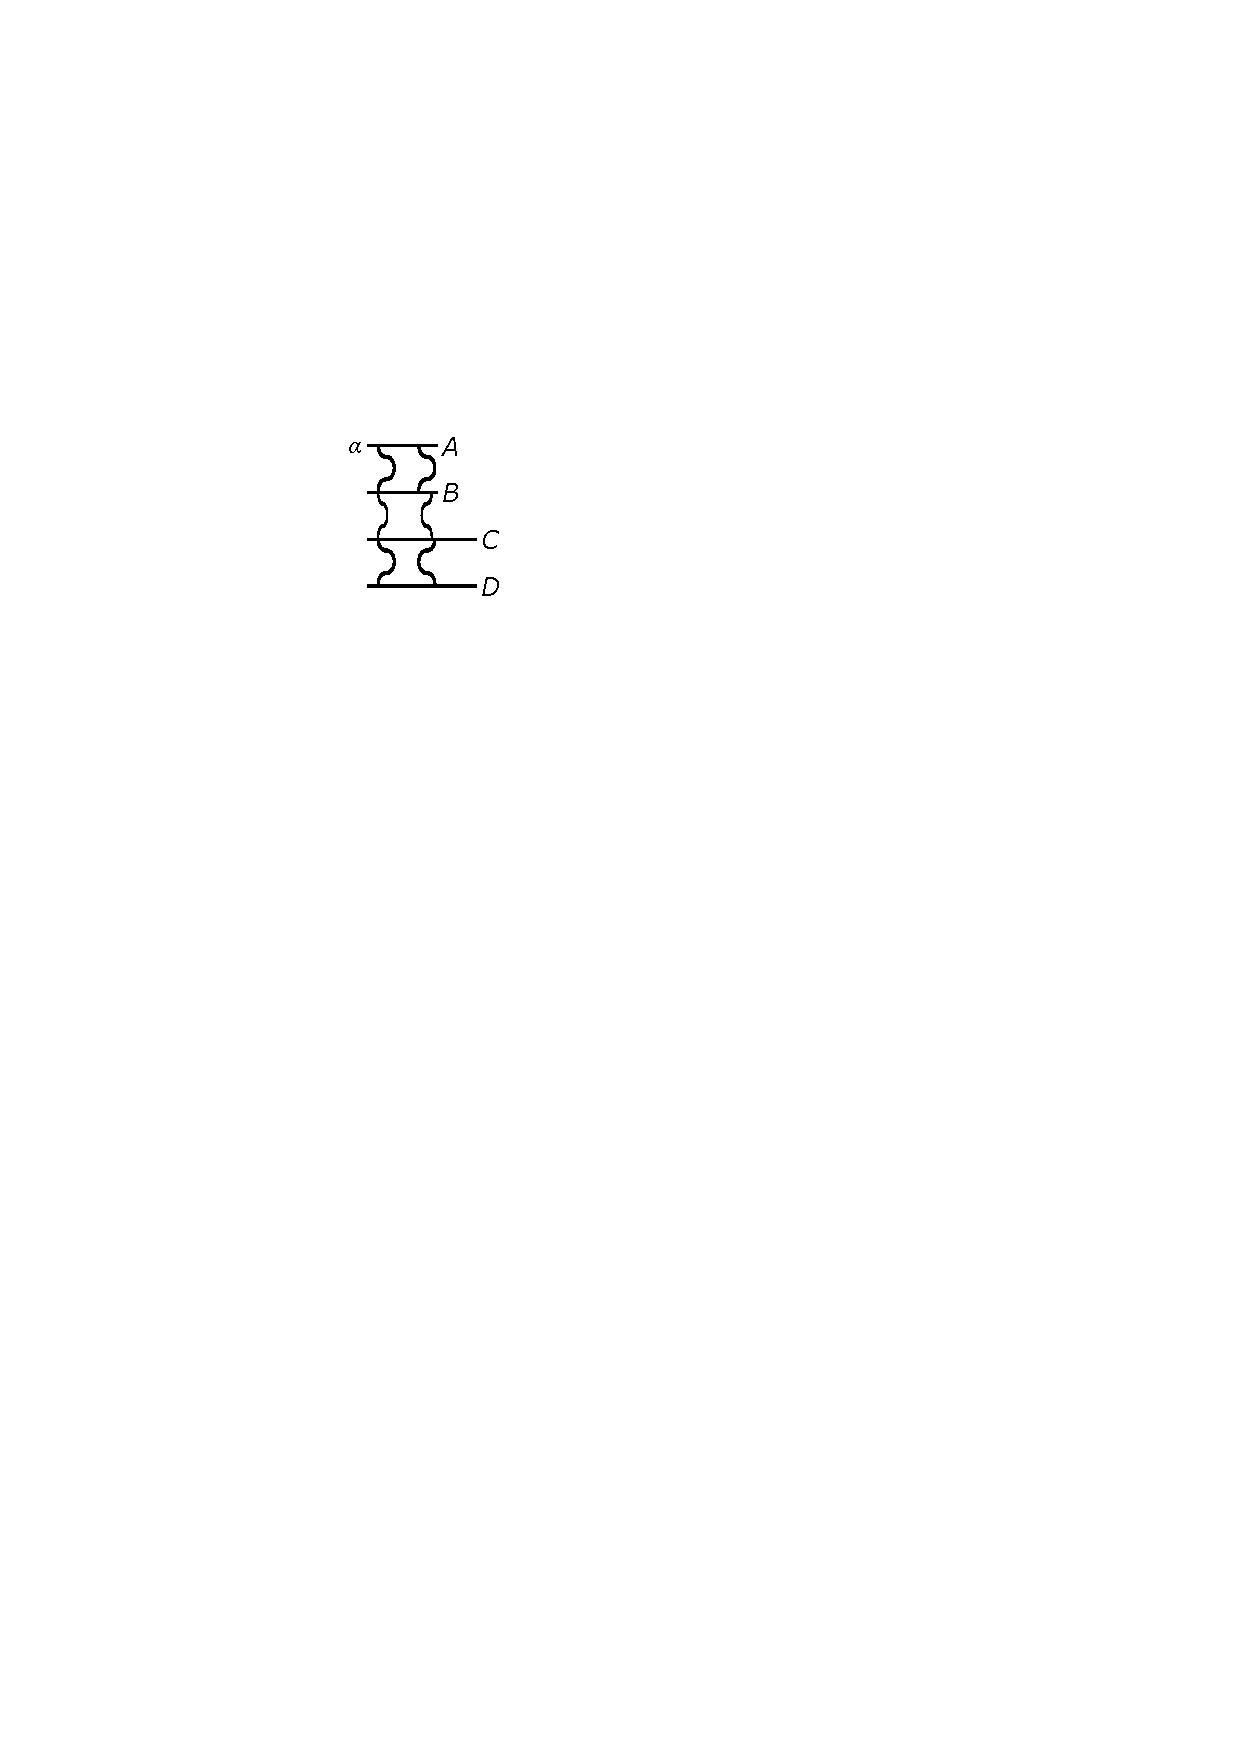
\includegraphics[width=0.16\textwidth]{gesamttex/edit_VIII-4/images/LH_37_04_160-161_d2_161r.pdf}
\edcaption[0.30em]%
{%
\lbrack\textit{Fig.\:2}\rbrack%
}%
\end{edfigure}%
\newpage%
\pstart%
Caeterum
\edtext{%
optima ratio hujus inventi%
\indexS{ratio inventi}%
\indexS{inventum}%
}{%
\lemma{optima}%
\Bfootnote{%
\textit{(1)}~rei %
\textit{(2)}~ratio hujus inventi%
~\textit{L}%
}}
est,
cum nec follibus %
nec ponderibus aliis opus
quam ipsa aqua.
Nimirum in Fodinis%
\indexS{fodina}
ex quibus aqua extrahi debet,%
\indexS{aqua extracta e fodinis}%
\indexS{extractio aquae e fodinis}
scilicet aqua vento extrahetur%
\indexS{aqua extracta vento}%
\indexS{ventus ad aquam extraendam}
maxima in copia
nec
\edtext{%
effund\lbrack e\rbrack tur%
}{%
\lemma{effundatur}%
\Bfootnote{%
\textit{L\;ändert Hrsg.}%
}}
inutiliter,
sed in ingentes lacus%
\indexS{lacus ingens}
\edtext{%
cond\lbrack e\rbrack tur,%
}{%
\lemma{condatur}%
\Bfootnote{%
\textit{L\;ändert Hrsg.}%
}}
unde postea ipsa
cessante vento%
\indexS{ventus cessans}
paulatim effluens
perpetui fluminis locum geret.%
\indexS{flumen perpetuum}%
\edlabel{LH_37_04_160-161_161r_molvent-2}
\pend%
\pstart%
Aliud
\edtext{%
est modus perennis Motus%
\indexS{motus perennis}%
}{%
\lemma{est}%
\Bfootnote{%
\textit{(1)}~motus %
\textit{(2)}~modus perennis Motus%
~\textit{L}%
}}
per simplex Barometrum,%
\indexS{barometrum simplex}
sed iisdem
quae dixi%
\lbrack:\rbrack\
follibus vel
\edtext{%
similibus.
Nam si habeat follis%
\indexS{follis adhibitus barometro}
latitudinem pedis,%
\indexS{pes}%
\indexS{latitudo follis}%
}{%
\lemma{similibus}%
\Bfootnote{%
\textit{(1)}~, si se %
\textit{(2)}~. Nam %
\textit{(a)}~qu %
\textit{(b)}~si %
\textit{(aa)}~diameter %
\textit{(bb)}~habeat %
\textit{(aaa)}~pedem %
\textit{(bbb)}~follem %
\textit{(ccc)}~follis latitudinem pedis,%
~\textit{L}%
}}
erit pondus aeris maximum%
\indexS{pondus aeris maximum}
Parisiis%
\indexO{Paris}
\edtext{%
1808 librarum,%
\indexS{libra Parisina}%
}{%
\lemma{1808}%
\Bfootnote{%
\textit{(1)}~pedum %
\textit{(2)}~librarum%
~\textit{L}%
}}
mediocre 1761 librarum,
minimum 1714 librarum,
differentia erit librarum 94 %
inter maximum et minimum,
et librarum 47 circiter inter minimum et mediocrem.
\edtext{%
\edlabel{LH_37_04_160-161_161r_marg-1}%
Ponamus autem
quovis mense non nisi ponderis decem librarum%
\indexS{libra Parisina}
esse differentiam,%
\indexS{differentia ponderis aeris}
\edtext{%
imo non nisi
vigesimam partem maximae differentiae,%
\indexS{differentia ponderis aeris}%
}{%
\lemma{imo non nisi}%
\Bfootnote{%
\bars{pondus \textit{streicht Hrsg.}}
\textit{(1)}~de %
\textit{(2)}~dicentesi %
\textit{(3)}~vigesimam partem maximae differentiae%
~\textit{L}%
}}
seu non nisi
circiter 5 librarum,
patet tamen
satis virium inesse 5 libris%
\indexS{libra Parisina}
ad motum perennem,%
\indexS{motus perennis}
qui (v.\,g.) horologio alicui circumagendo
\edlabel{LH_37_04_160-161_161r_dae_1a}%
sufficiat.%
\edlabel{LH_37_04_160-161_161r_marg-2}%
}{%
\lemma{\textit{Vom Text umrandet:}}%
\Afootnote{%
1 pouce pollex quorum 12 faciunt talem pedem.%
\textsuperscript{\lbrack a\rbrack}%
\indexS{pouce}%
\indexS{pollex}%
\indexS{pes Parisinus}%
\\[1ex]%
{\footnotesize%
\textsuperscript{\lbrack a\rbrack}~%
1 pouce \lbrack...\rbrack\ pedem:
Der inhaltliche Bezugspunkt ist wohl \refpassage{LH_37_04_160-161_161v_sgi-1}{LH_37_04_160-161_161v_sgi-2}.%
}%
}}%
\edtext{}{%
\xxref{LH_37_04_160-161_161r_dae_1a}{LH_37_04_160-161_161r_dae_1b}%
\lemma{sufficiat.}%
\Bfootnote{%
\textit{(1)}~\lbrack/\rbrack\ Tertium principi %
\textit{(2)}~An id %
\lbrack...\rbrack\ motus principium%
~\textit{L}%
}}
\edtext{%
An id ad horologium portabile%
\indexS{horologium portabile}
applicari possit postea videbimus.%
}{%
\lemma{An id \lbrack...\rbrack\ videbimus}%
\Cfootnote{%
Vgl. \refpassage{LH_37_04_160-161_161v_postea}{LH_37_04_160-161_161v_postea}.%
}}
\pend%
\pstart%
Tertium motus principium%
\indexS{principium motus}%
\edlabel{LH_37_04_160-161_161r_dae_1b}
est calor%
\indexS{calor principium motus}
seu thermometrum.%
\indexS{thermometrum}
Et quidem ponamus
calore effici%
\indexS{calor dilatans aerem}
ut aer conetur locum occupare%
\indexS{aer conans occupare locum}
qui sit ad
\edtext{%
priorem
ut 10 %
ad \lbrack 9\rbrack\ idque%
}{%
\lemma{priorem ut}%
\Bfootnote{%
\textit{(1)}~9 ad %
\textit{(2)}~10, ad %
\bars{9 \textit{erg.\;Hrsg.\;nach \refpassage{LH_37_04_160-161_161v_fui-1}{LH_37_04_160-161_161v_fui-2}.}} idque%
~\textit{L}%
}}
nisi impediatur
effecturum esse,
patet non tantum
hanc vim praeponderare aeris massae,%
\indexS{vis praeponderans massae aeris}%
\indexS{massa aeris}
alioqui enim eam non elevaret,
sed et duci debere in quantitatem extensionis,
ut habetur vis ista.
Cumque quotidie contingat haec mutatio,%
\indexS{mutatio contingens}
\lbrack%
\href{\Scan{LH_37_04_161v}}%
{161\,v\textsuperscript{o}}%
\rbrack\
fere
\edtext{%
enim noctes%
\indexS{nox frigidior die}
diebus%
\indexS{dies}%
}{%
\lemma{enim}%
\Bfootnote{%
\textit{(1)}~dies noctibus %
\textit{(2)}~noctes diebus%
~\textit{L}%
}}
frigidiores esse solent.
Ideo credibile est
satis magnam hoc modo vim suppeditari forte%
\indexS{vis suppeditans}
et ad molendinum mediocre circumagendum ope follis.%
\indexS{vis ad molendinum circumagendum}%
\indexS{molendinum circumagendum ope follis}%
\indexS{follis ad circumagendum molendinum}
Crebritas enim harum mutationum%
\indexS{crebritas mutationum}
debilitatem large compensat.
Tantum ergo aer communis folli inclusus esse debet.%
\indexS{aer communis}%
\indexS{aer inclusus folli}
\pend%
\newpage%
\pstart%
Quartum principium%
\indexS{principium motus}
erit siccitas%
\indexS{siccitas principium motus}
et humiditas%
\indexS{humiditas principium motus}
seu hygrometrum%
\indexS{hygrometrum principium motus}
quod magnam etiam vim%
\indexS{vis hygrometri}
habere patet
inprimis ex eleganti illo
\edtext{%
Hygrometro ligneo,%
\indexS{hygrometrum ligneum}
quod in eruditorum diario describitur.%
}{%
\lemma{Hygrometro \lbrack...\rbrack\ describitur}%
\Cfootnote{%
Siehe
\glqq Extrait du Journal d'Angleterre, contenant la description et la figure d'un hygroscope pour mesurer les degrez de l'humidité et de la seicheresse de l'air\grqq\
(\textit{JS}, 15.\;März 1677, S.\;68--70).\cite{01473}
Der anonyme Auszug entstammt folgender, ebenfalls anonymer Mitteilung:
\glqq An extract of a letter written from Dublin, containing divers particulars of a philosophical nature\grqq\
(\textit{PT} XI, 18.\;Juli 1676, S.\;650--652 u. Tafel~I).\cite{01474}%
}}
Quod ad parva utile foret,
ad magna autem ingentes corrigiae ex corio%
\indexS{corrigia secta e corio}%
\indexS{corium}
imbuto sectae,
\edtext{%
quae facile humiditatem%
\indexS{humiditas exuta corio}
trahunt exuuntque.%
}{%
\lemma{quae}%
\Bfootnote{%
\textit{(1)}~faciunt aut %
\textit{(2)}~facile humiditatem trahunt exuuntque%
~\textit{L}%
}}
Fateor tamen
mutationes%
\indexS{mutatio humiditatis}%
\indexS{mutatio siccitatis}
humiditatis%
\indexS{humiditas mutans}
siccitatisque%
\indexS{siccitas mutans}
quibusdam anni tempestatibus%
\indexS{tempestas anni}%
\indexS{annus}
non satis crebro contingere.
\pend%
\pstart%
\edlabel{LH_37_04_160-161_161v_postea}%
Venio jam ad Horologii portatilis elaborationem,%
\indexS{horologium portatile}%
\indexS{elaboratio horlogii portatilis}
quod duorum pollicum diametri sit ad summum.%
\indexS{pollex}
Jungenda hic in unum arbitror Thermometrum,%
\indexS{thermometrum junctum horologio portatili}
Barometrum%
\indexS{barometrum junctum horologio portatili}
et Hygrometrum.%
\indexS{hygrometrum junctum horologio portatili}
Scilicet unumquodque ex ipsis adjunctum sibi habebit suum elaterium,%
\indexS{elaterium thermometri}%
\indexS{elaterium barometri}%
\indexS{elaterium hygrometri}
quod agente
\edtext{%
calore,%
\indexS{calor agens}
aeris pondere,%
\indexS{pondus aeris agens}
humiditate,%
\indexS{humiditas agens}
cedit%
\indexS{elaterium cedens}%
}{%
\lemma{calore,}%
\Bfootnote{%
\textit{(1)}~sive humid %
\textit{(2)}~aeris pondere, humiditate, %
\textit{(a)}~ad %
\textit{(b)}~cedit%
~\textit{L}%
}}%
\lbrack,\rbrack\
ea autem remittente se%
\indexS{elaterium restituens se}
\edtext{%
restituit.
Rota autem aliqua%
\indexS{rota horologii}%
}{%
\lemma{restituit.}%
\Bfootnote{%
\textit{(1)}~Quando autem %
\textit{(a)}~prorsum %
\textit{(b)}~prorsus et ratio %
\textit{(2)}~Rota autem aliqua%
~\textit{L}%
}}
his reciprocationibus%
\indexS{reciprocatio elaterii}
semper agetur in eandem partem.%
\indexS{rota acta semper in eandem partem}
Talis rota cuilibet %
harum virium separatim additur.%
\indexS{vis elaterii}
Unaquaeque ex his rotis aget
in Elaterium Horologii a tergo,%
\indexS{elaterium horologii}%
\indexS{horologium portatile}
id est ipsum tendendo ut in pendulis,%
\indexS{pendulum}
quia si ab altera parte tendatur,
nil turbatur pendulum.
Plures istae rotae%
\indexS{rota horologii}
se invicem juvare poterunt,
imo et una sine alia agere,
quod ut fiat
commodius opus erit
rotam magnam aliquam ipsi Elaterio affixam%
\indexS{rota affixa elaterio horologii}%
\indexS{elaterium horologii}
esse sectam in maximum numerum dentium exiguorum%
\indexS{dentes rotae}
in unam tantam partem inclinatorum,
ita %
ut non detur retroitus.%
\indexS{retroitus rotae}
Ita vel minimus conatus efficiet aliquid%
\indexS{conatus minimus}%
\lbrack,\rbrack\
et quando se simul jungent rotae%
\indexS{rota horologii}
minus resistet Elaterium.%
\indexS{elaterium resistens}%
\indexS{resistentia elaterii}
\pend%
\pstart%
Restat tamen hoc desiderandum,%
\indexS{desiderandum}
ut Elaterium%
\indexS{elaterium horologii}
eo ducatur longius,%
\indexS{elaterium ductum longius}
quo a pluribus premitur,
quod hic non fit.
Sed his remedium in%
\indexS{remedium}
\edtext{%
promtu.
\edlabel{LH_37_04_160-161_161v_fltherm}%
Puto commodissimum Thermometrum%
\indexS{thermometrum calefactum in marsupio}%
\indexS{thermometrum refrigeratum noctu}
quia%
}{%
\lemma{promtu.}%
\Bfootnote{%
\textit{(1)}~Elaterium %
\textit{(2)}~Puto commmodissimum %
\textit{(a)}~quia %
\textit{(b)}~Thermometrum quia%
~\textit{L}%
}}
noctu diuque magna mutatio est,%
\indexS{mutatio thermometri}
praeterea
\edtext{%
dum gestatur in marsupio%
\indexS{marsupium}%
}{%
\lemma{dum}%
\Bfootnote{%
\textit{(1)}~gerit %
\textit{(2)}~gestatur in %
\textit{(a)}~mas %
\textit{(b)}~marsupio%
~\textit{L}%
}}
valde calefit,
noctu iterum refrigeratur.%
\indexS{nox}
Praeterea quis facile divinaret%
\lbrack?\rbrack\
tantum enim efficiendum
ut exigua quaedam foraminula sint%
\indexS{foraminulum exiguum}
\edtext{%
obturata,
claudentia Thermometri follem,%
\indexS{follis thermometri}
at si%
}{%
\lemma{obturata,}%
\Bfootnote{%
\textit{(1)}~quae si %
\textit{(2)}~claudentia Thermometri follem, at si%
~\textit{L}%
}}
quis manu contingat%
\indexS{manus}%
\indexS{contactus manus}
et inspicere artificium velit,%
\indexS{artificium inspectum}
effici potest,
ut minimis quibusdam indiculis remotis ac perditis
foramen maneat,%
\indexS{foramen exiguum}
valde exiguum licet,
aliquod tamen,
et facile efficiemus
ut nec vestigium indiculae maneat %
et locus foraminis transformetur,
quo facto
non video
quomodo rem aliquis facile divinare
\edtext{%
possit.
\edlabel{LH_37_04_160-161_161v_folfer-1}%
Follis sit%
}{%
\lemma{possit.}%
\Bfootnote{%
\textit{(1)}~Sit %
\textit{(2)}~Follis sit%
~\textit{L}%
}}
totus ferreus,%
\indexS{follis ferreus}
id est pro corio%
\indexS{corium}
laminae ferreae%
\indexS{lamina ferrea}
\edtext{%
elasticae,%
\indexS{lamina elastica}
igne%
\indexS{ignis}
tabulis junctae,%
\indexS{tabula thermometri}
ita nullus est%
}{%
\lemma{elasticae,}%
\Bfootnote{%
\textit{(1)}~igne jungentes ita nullus fu %
\textit{(2)}~igne tabulis %
\lbrack...\rbrack\ nullus est%
~\textit{L}%
}}
metus aeris penetraturi.%
\indexS{metus aeris penetraturi}%
\indexS{aer penetraturus}%
\edlabel{LH_37_04_160-161_161v_folfer-2}
\pend%
\pstart%
Quantum ad quantitatem virium%
\indexS{quantitas virium}
in exiguo datarum,%
\indexS{vis data in exiguo}
ita ratiocinabimur.
\edtext{%
\edlabel{LH_37_04_160-161_161v_sgi-1}%
Aeris massa imminens%
\indexS{massa aeris imminens}%
\indexS{aer imminens}
circulo%
\indexS{circulus}
\edtext{%
diametri%
\indexS{diameter circuli}
pollicis%
\indexS{pollex}
est circiter 12 librarum,%
\edlabel{LH_37_04_160-161_161v_sgi-2}%
}{%
\lemma{diametri}%
\Bfootnote{%
\textit{(1)}~(\phantom)\hspace*{-1.5mm}pedalis esse circiter 7 librarum %
\textit{(2)}~duorum pollicum %
\textit{(3)}~pollicis est circiter 12 librarum,%
~\textit{L}%
}}%
}{%
\lemma{Aeris \lbrack...\rbrack\ librarum}%
\Cfootnote{%
Vgl. \refpassage{LH_37_04_160-161_161r_pasca-1}{LH_37_04_160-161_161r_pasca-2}.
Zu beachten ist, dass ein Fuß zwölf Zoll entspricht, wie in der Randbemerkung zu \refpassage{LH_37_04_160-161_161r_marg-1}{LH_37_04_160-161_161r_marg-2} festgestellt.%
}}
\indexS{libra}
et si diameter%
\indexS{diameter circuli}
sit 2 pollicum%
\indexS{pollex}
erit circiter 48
\edtext{%
librarum.
Ergo Aeris%
}{%
\lemma{librarum.}%
\Bfootnote{%
\textit{(1)}~Itaque calor qui aerem %
\textit{(2)}~Ergo Aeris%
~\textit{L}%
}}
apud nos%
\indexS{aer apud nos}
in naturali statu constituti%
\indexS{aer constitutus in statu naturali}%
\indexS{status naturalis}
vis%
\indexS{vis aeris communis}
seu Elaterium%
\indexS{elaterium aeris communis}
est 48 librarum.%
\indexS{libra}
Quicquid aerem apud nos%
\indexS{aer apud nos}
rarefacere est,%
\indexS{aer rarefactus}
id majorem vim%
\indexS{vis aeris communis}
habere necesse est,
et attollere totum aeris cylindrum,%
\indexS{cylinder aeris}
et in tantum quidem,
in quantum magis rarefacit.
Hoc ita intelligendum%
\lbrack:\rbrack\
Elastrum aeris%
\indexS{elastrum aeris}
et cylinder massae aereae%
\indexS{cylinder massae aereae}%
\indexS{massa aerea}
sunt in aequilibrio,%
\indexS{aequilibrium inter elastrum et massam aeris}
ergo exiguus calor superveniens%
\indexS{calor superveniens}
facit,
ut alterum vincat,
scil.\;Elastrum.%
\indexS{elastrum aeris}
Cum autem aer%
\indexS{aer rarefactus calore}%
\indexS{rarefactio aeris}
calore rarefit,%
\indexS{calor rarefaciens aerem}
perinde esse arbitror
ac si ob condensationem rarefieret,%
\indexS{rarefactio aeris ob condensationem}%
\indexS{condensatio aeris}
nam idem est effectus%
\indexS{effectus rarefactionis aeris}%
\lbrack;\rbrack\
ut si aer%
\indexS{aer conans occupare plus spatium}
calore%
\indexS{calor dilatans aerem}
duplo majus occupare spatium conetur,
perinde erit,
ac si
ob nimiam condensationem%
\indexS{condensatio aeris}
duplo majus spatium occupare quaereret.%
\indexS{aer quaerens occupare plus spatium}
Nam quorum effectus idem%
\indexS{effectus idem quam vis}
eorum vis eadem%
\indexS{vis eadem quam effectus}%
\lbrack;\rbrack\
\edlabel{LH_37_04_160-161_161v_fui-1}
quod si spatium aeris calefacti%
\indexS{spatium aeris calefacti}%
\indexS{aer calefactus}%
\indexS{calefactio aeris}
ad spatium ordinarii%
\indexS{spatium aeris ordinarii}%
\indexS{aer ordinarius}
ut 10 ad 9,
etiam vis%
\indexS{vis aeris calefacti}
\edtext{%
erit
$\displaystyle\frac{1}{9}$
vis ordinariae%
\indexS{vis aeris ordinaria}%
}{%
\lemma{erit}%
\Bfootnote{%
\textit{(1)}~$\displaystyle\frac{1}{10}$ vis ordinariae %
\textit{(2)}~$\displaystyle\frac{1}{}$ %
\textit{(3)}~$\displaystyle\frac{1}{9}$ vis ordinariae%
~\textit{L}%
}}
seu%
\rule[-0mm]{0pt}{4.4mm}
$\displaystyle\frac{1}{9}$
pressionis atmosphaerae,%
\indexS{pressio atmosphaerae}%
\indexS{atmosphaera}
seu
$\displaystyle\frac{1}{9}$
\edtext{%
librarum 48,%
\indexS{libra}%
\edlabel{LH_37_04_160-161_161v_fui-2}
quod est pondus aeris%
\indexS{pondus aeris premens in diametrum duorum pollicum}
in diametrum duorum pollicum prementis,%
}{%
\lemma{librarum 48}%
\Bfootnote{%
\textit{(1)}~in duos pollices %
\textit{(2)}~quod est %
\lbrack...\rbrack\ pollicum prementis,%
~\textit{L}%
}}
id est librarum 5,%
\indexS{libra}%
\rule[-0mm]{0pt}{3.3mm}
quod pondus horologio portatili%
\indexS{horologium portatile}
aliquot diebus sufficit.%
\indexS{dies}
\pend%
\pstart%
Pulcherrima quaestio,%
\indexS{quaestio pulcherrima}
et hic utilis,%
\indexS{quaestio utilis}
an aer compressus%
\indexS{aer compressus}
ab eodem%
\indexS{calor dilatans aerem}
\textls{calore}
majorem se dilatandi conatum \textls{novum} accipiat%
\indexS{conatus novus}%
\indexS{conatus acceptus}%
\indexS{conatus major}%
\indexS{conatus aeris dilatandi se}%
\indexS{conatus aeris compressi}
quam aer ordinarius%
\indexS{aer ordinarius}%
\indexS{conatus aeris ordinarii}
vel rarus.%
\indexS{aer rarus}%
\indexS{conatus aeris rari}
Ita credo,
quia aer rarissimus,%
\indexS{aer rarus}
ob calorem fere nihil efficiet,
seu calore%
\indexS{calor dilatans aerem}
\textlangle\textendash\ \textendash\ \textendash\ imo\textrangle\ eruitur,
ut ille%
\indexS{aer in loco prope vacuo}
qui in loco prope vacuo est.%
\indexS{locus prope vacuus}
\pend%
\selectlanguage{latin}%
\frenchspacing%
\normalsize%
